\section{Kombinatorik}
\label{sec:Kombinatorik}
Um bei Laplace-Versuchen die Wahrscheinlichkeit eines Ereignisses zu berechnen, muss man die Anzahl günstige und mögliche Fälle bestimmen. Sind diese Zahlen sehr gross, kann das Zählen schwierig sein. Wir benötigen daher Regeln und günstige Abzählverfahren. Die Kunst und Theorie des Zählens nennt man \emph{Kombinatorik}.

\subsection{Der Multiplikationssatz}

Im Grunde lassen sich alle Fragen der Kombinatorik mit einem einzigen Prinzip lösen: Dem \emph{Multiplikationssatz} bzw. mit dem Baumprinzip.

Ein Mädchen besitzt zwei Hüte, vier Kleider und drei Paar Schuhe. Zu wie vielen verschiedenen Outfits kann es ihre Kleider kombinieren?

Dass man hier einfach nur multiplizieren muss, sieht man am \emph{Baumdiagramm}. Auf die Reihenfolge der Multiplikation kommt es dabei nicht an.

\begin{minipage}{0.25\textwidth}
    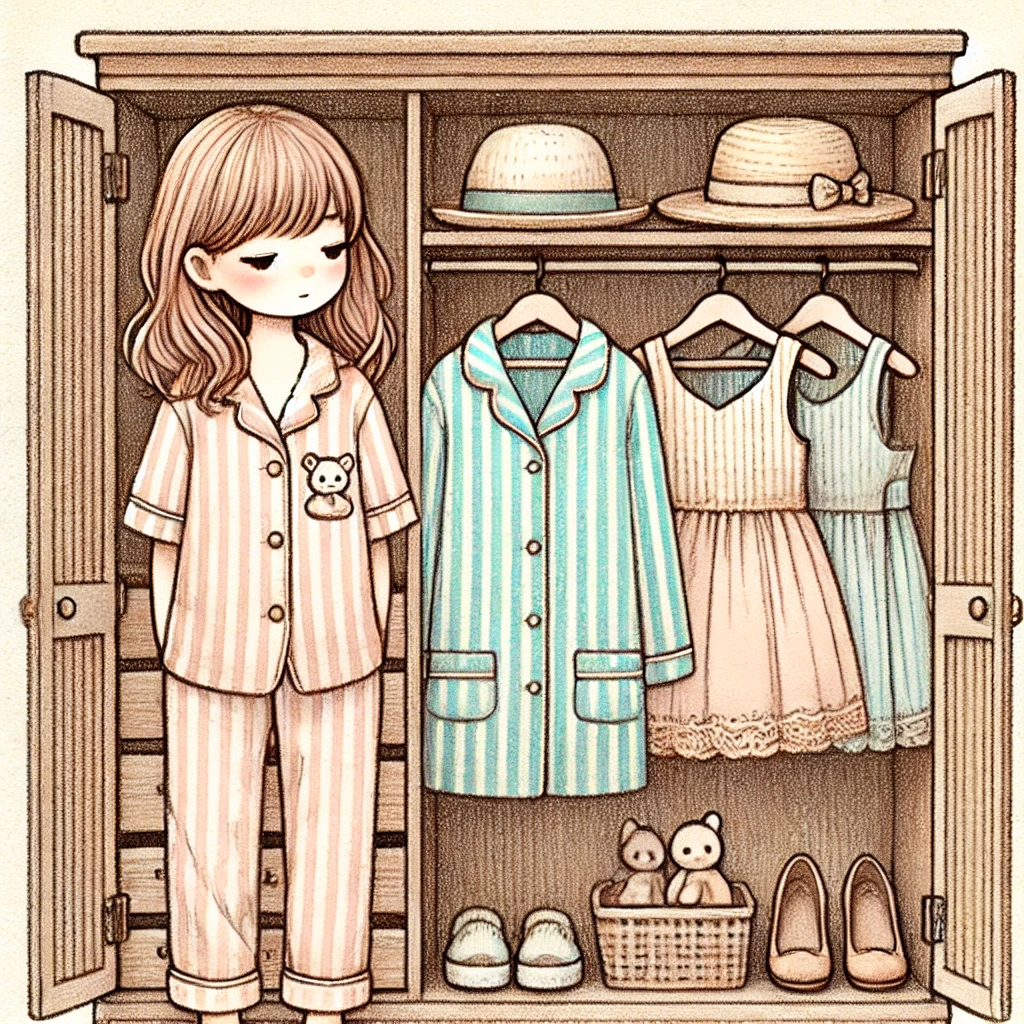
\includegraphics[width=\textwidth]{media/garderobe.png}
    \captionsetup{hypcap=false}
    \captionof{figure}{\footnotesize{Bild mit DALL.E erstellt}}
    \label{garderobe}
\end{minipage}
\hspace{0.05\textwidth}
\begin{minipage}{0.7\textwidth}






    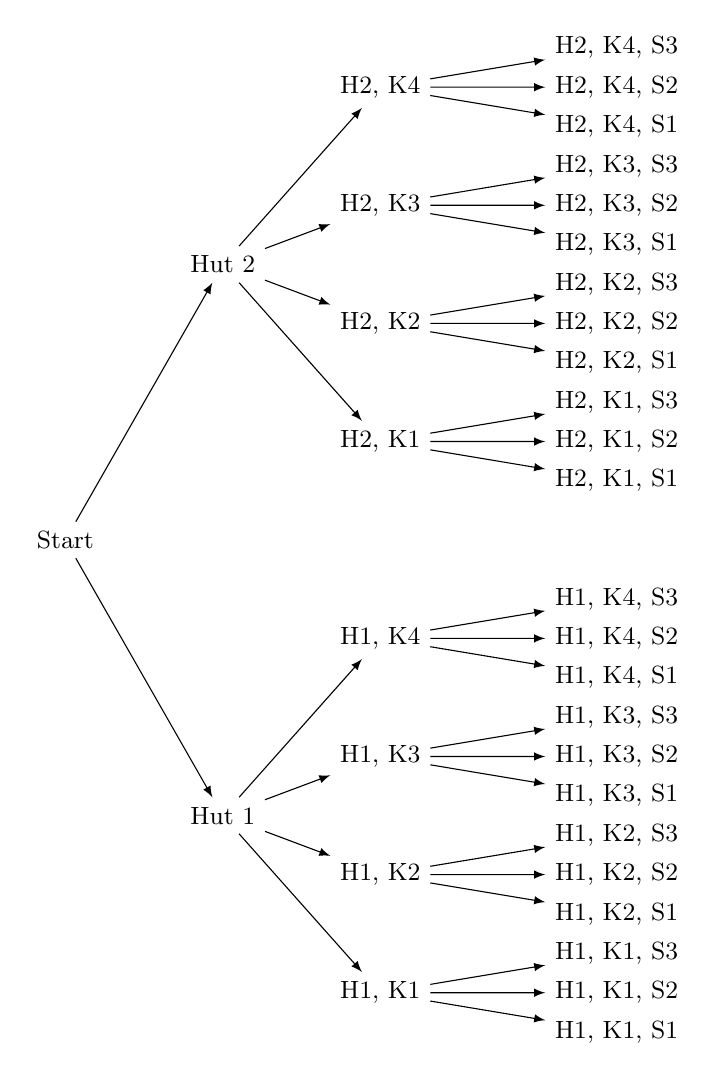
\begin{tikzpicture}[
            grow=east,
            level 1/.style={sibling distance=7cm, level distance=2cm},
            level 2/.style={sibling distance=1.5cm, level distance=2cm},
            level 3/.style={sibling distance=0.5cm, level distance=3cm},
            edge from parent/.style={draw, -latex},
            every node/.style={font=\small},
        ]

        % Root node
        \node {Start}
        % First level: Hüte
        child { node {Hut 1}
                % Second level: Kombinationen aus Hut 1 und Kleidern
                child { node { H1, K1}
                        % Third level: Kombinationen aus Hut 1, Kleid 1 und Schuhen
                        child { node {H1, K1, S1} }
                        child { node {H1, K1, S2} }
                        child { node {H1, K1, S3} }
                    }
                child { node {H1, K2}
                        child { node {H1, K2, S1} }
                        child { node {H1, K2, S2} }
                        child { node {H1, K2, S3} }
                    }
                child { node {H1, K3}
                        child { node {H1, K3, S1} }
                        child { node {H1, K3, S2} }
                        child { node {H1, K3, S3} }
                    }
                child { node {H1, K4}
                        child { node {H1, K4, S1} }
                        child { node {H1, K4, S2} }
                        child { node {H1, K4, S3} }
                    }
            }
        child { node {Hut 2}
                % Second level: Kombinationen aus Hut 2 und Kleidern
                child { node {H2, K1}
                        child { node {H2, K1, S1} }
                        child { node {H2, K1, S2} }
                        child { node {H2, K1, S3} }
                    }
                child { node {H2, K2}
                        child { node {H2, K2, S1} }
                        child { node {H2, K2, S2} }
                        child { node {H2, K2, S3} }
                    }
                child { node {H2, K3}
                        child { node {H2, K3, S1} }
                        child { node {H2, K3, S2} }
                        child { node {H2, K3, S3} }
                    }
                child { node {H2, K4}
                        child { node {H2, K4, S1} }
                        child { node {H2, K4, S2} }
                        child { node {H2, K4, S3} }
                    }
            };

    \end{tikzpicture}

\end{minipage}



\clearpage
\begin{ueb}
    {Zum Multiplikationssatz}{}
    \begin{enumerate}
        \item Wie viele 5-stellige Zahlen kann man unter ausschliesslicher Verwendung der Ziffern 1, 2, 3 bilden?

        \item Eine Firma verkauft den Bürostuhl ``Capo'' in 3 verschiedenen Grössen und in 6 verschiedenen Farben. Ferner kann der Kunde wählen, ob der Stuhl fahrbar sein soll oder nicht. Wie viele verschiedene Bürostühle des Modells ``Capo'' bietet die Firma zum Verkauf an?

        \item In einem französischen Restaurant werden bei einem Menü mit 4 Gängen Auswahlmöglichkeiten angeboten:
              \begin{itemize}
                  \item zuerst ein Salat oder eine Suppe,
                  \item anschliessend 4 verschiedene Vorspeisen,
                  \item 3 Hauptspeisen und
                  \item 5 Desserts.
              \end{itemize}
              Wie viele Bestellmöglichkeiten gibt es, wenn kein Gang ausgelassen wird?

        \item Ein Sportgeschäft verkauft Schlittschuhe für Damen und für Herren in je 2 Qualitäten und 20 verschiedenen Schuhgrössen. Wie viele Schlittschuhpaare muss das Geschäft am Lager haben, wenn jedes mögliche Paar dreifach vorhanden sein soll?

        \item Ein Morse-Zeichen wird mit Punkten und Strichen gebildet.
              \begin{enumerate}
                  \item Wie viele 3-stellige Morsezeichen sind möglich?
                  \item Wie viele höchstens 4-stellige Morsezeichen sind möglich?
              \end{enumerate}

        \item Auf einem Parkplatz sind noch 6 Parkplätze frei. Gleichzeitig kommen
              \begin{enumerate}
                  \item 3 Autos an,
                  \item 5 Autos an,
                  \item 6 Autos an.
                  \item 8 Autos an.
              \end{enumerate}
              Wie viele Möglichkeiten gibt es, die freien Parkplätze den ankommenden Autos zuzuweisen?

        \item 4 Personen treten in einen Raum mit 7 Stühlen, die fest montiert sind. Wie viele Sitzordnungen sind denkbar?

        \item Die Ziffern einer Zahl sollen durch Werfen eines Würfels bestimmt werden. Wie viele verschiedene 4-stellige Zahlen sind denkbar?

        \item Wie viele 5-stellige
              \begin{enumerate}
                  \item Zahlen mit lauter ungeraden Ziffern gibt es?
                  \item ungerade Zahlen gibt es?
                  \item Zahlen mit lauter verschiedenen Ziffern gibt es?
                  \item Zahlen mit lauter verschiedenen ungeraden Ziffern gibt es?
                  \item Zahlen mit lauter geraden Ziffern gibt es?
                  \item gerade Zahlen gibt es?
                  \item Zahlen mit lauter verschiedenen geraden Ziffern gibt es?
              \end{enumerate}

        \item Wie viele ``Wörter'', bestehend aus 7 Buchstaben, kann ein Computer aufschreiben, wenn das Alphabet 26 Buchstaben hat? Wie lange braucht er dazu, wenn er pro Sekunde ein solches ``Wort'' schreiben kann?
    \end{enumerate}

\end{ueb}
\clearpage
\textbf{Lösungen}
\begin{enumerate}
    \item 243
    \item 36
    \item 120
    \item 240
    \item 20160
          \begin{enumerate}
              \item 8
              \item 30
          \end{enumerate}
    \item
          \begin{enumerate}
              \item 120
              \item 720
              \item 720
              \item
          \end{enumerate}
    \item 840
    \item 1296
    \item
          \begin{enumerate}
              \item 3125
              \item 45\,000
              \item 27\,216
              \item 120
              \item 2500
              \item 45\,000
              \item 96
          \end{enumerate}
    \item
          \begin{enumerate}
              \item 8\,031\,810\,176
              \item 254.7 Jahre
          \end{enumerate}
\end{enumerate}

\clearpage
\subsection{Das Urnenmodell}

Fast alle Probleme der Kombinatorik lassen sich auf das sogenannte \emph{Urnenmodell} zurückführen. Wie das im Einzelnen geht, werden Sie später an vielen Beispielen sehen. Zunächst wollen wir erst einmal das Urnenmodell kennenlernen.

In einer Urne liegen \(n\) verschiedene Kugeln. Davon werden \(k\) gezogen. Man unterscheidet zwischen den folgenden Zugtechniken:
\begin{itemize}
    \item Nach jeder Ziehung wird die gezogene Kugel entweder zurück in die Urne gelegt, oder nicht.

          Kurz: Mit/Ohne Wiederholung
    \item Entweder kommt es auf die Reihenfolge der gezogenen Kugeln an, oder nicht.

          Kurz: Mit/Ohne Reihenfolge
\end{itemize}

Insgesamt gibt es also vier Arten, wie man die Kugeln ziehen kann. Im Folgenden werden wir für jede Art des Ziehens eine Formel für die Anzahl Möglichkeiten herleiten.

\subsubsection{Ziehen mit Wiederholung und mit Berücksichtigung der Reihenfolge}
Aus einer Urne mit \(n\) verschiedenen Kugeln zieht man \(k\)-mal eine Kugel \textbf{mit Zurücklegen}. Notiert man nach jedem Zug die Nummer der gezogenen Kugel, erhält man ein geordnetes \(k\)-Tupel.

Mögliche Resultate für \(n = 10\) und \(k = 4\) wären z.\,B.
\[
    (4,7,2,7) \quad \text{oder} \quad (3,4,10,1).
\]

\begin{satz}
    {Geordnete Stichprobe mit Wiederholung}{}
    Aus einer Menge mit \(n\) verschiedenen Elementen kann man

    \vspace{2cm}

    geordnete Stichproben mit Wiederholung vom Umfang \(k\) entnehmen.

\end{satz}

\begin{bsp}
    {Fussballtoto}{}
    Beim Fussballtoto muss der Spielausgang von 13 Fussballspielen vorausgesagt werden. Dabei kreuzt man bei jedem Spiel eine 0, 1 oder 2 an. Dabei bedeutet:
    \begin{itemize}
        \item 0: Unentschieden,
        \item 1: Sieg der Heimmannschaft,
        \item 2: Sieg der Gastmannschaft.
    \end{itemize}

    \begin{enumerate}
        \item Auf wie viele Arten kann man einen Totoschein ausfüllen?
              \vspace{2cm}
        \item Mit welcher Wahrscheinlichkeit gewinnt man den Jackpot, wenn man den Totoschein zufällig ausfüllt?
              \vspace{2cm}
    \end{enumerate}
\end{bsp}

\begin{bsp}{Urne = Kugel?}{}
    Dreizehn verschiedene Kugeln werden auf zwei Urnen zufällig verteilt. Dabei kann eine Urne beliebig viele Kugeln aufnehmen. Wie viele verschiedene Kugelverteilungen sind möglich?

    \vspace{2cm}
\end{bsp}

\begin{bsp}
    {Münze werfen}{}
    Eine Laplace-Münze wird \(k\)-mal geworfen und das Resultat (K oder Z) notiert.

    \begin{enumerate}
        \item Wie viele Resultate sind denkbar?
              \vspace{2cm}
        \item Wie häufig muss man eine Münze werfen, damit die Wahrscheinlichkeit, dass immer Zahl erscheint, kleiner als 1\% ist?
              \vspace{4cm}
    \end{enumerate}
\end{bsp}


















\subsubsection{Ziehen ohne Wiederholung und mit Berücksichtigung der Reihenfolge}
Zunächst betrachten wir einen Spezialfall – die Permutationen: Aus einer Urne mit \(n\) Kugeln werden ohne Zurücklegen der Reihe nach alle Kugeln gezogen. Notiert man nach jedem Zug die Nummer der gezogenen Kugel, erhält man ein geordnetes \(n\)-Tupel ohne Wiederholung.

Mögliche Resultate für \(n=4\) wären \((1,2,4,3)\) oder \((2,3,4,1)\). \\

Anzahl möglicher Ausfälle für \(n=4\): \\

Damit man nicht immer alle Faktoren aufschreiben muss, hat man für diese Art Produkte eine abkürzende Schreibweise eingeführt:

\begin{definition}
    {Fakultät}{}
    Sei \(n\in\N\) das Produkt

    \vspace{1cm}

    nennt man \(n\) \emph{Fakultät}. Man schreibt dafür \(n!\)\\
    Spezialfall: Es gilt \(0! = 1\)
\end{definition}

Kommen wir nun zum allgemeinen Fall:\\
Aus einer Urne mit \(n\) Kugeln wird \(k\)-mal eine Kugel ohne Zurücklegen gezogen. Notiert man nach jedem Zug die Nummer der gezogenen Kugel, erhält man ein \(k\)-Tupel ohne Wiederholung.

Mögliche Resultate für \(n=10\) und \(k=4\) wären \((9,3,7,2)\) oder \((10,1,3,6)\).

Anzahl der möglichen Ausfälle für \(n=10\) und \(k=4\): \\\\

\begin{satz}
    {Geordnete Stichprobe ohne Wiederholung}{}
    Aus einer Menge mit \(n\) Elementen kann man

    \vspace{2cm}

    geordnete Stichproben ohne Wiederholung vom Umfang \(k\) entnehmen.
\end{satz}


\begin{bsp}
    {}{}
    An einem 100m-Lauf nehmen 10 Schülerinnen teil. Auf wie viele Arten können die Medaillenplätze belegt werden?

    \vspace{1cm}

\end{bsp}

\begin{bsp}
    {}{}
    Auf einem Tisch liegen 26 Karten, deren Rückseite die 26 Buchstaben des Alphabets tragen. Fünf Karten werden umgedreht. Wie viele Wörter (auch sinnlose) kann man erzeugen? \\
    Mit welcher Wahrscheinlichkeit ist das Wort ``MATHE'' entstanden?


    \vspace{2cm}

\end{bsp}

\begin{bsp}
    {}{}
    Sechs Personen setzen sich nebeneinander auf eine Bank. Wie viele Anordnungen sind möglich?

    \vspace{2cm}

\end{bsp}

\begin{ueb}
    {}{}
    \begin{enumerate}
        \item Vereinfachen Sie:
              \begin{enumerate}
                  \item \(12 \cdot 11!\)
                  \item \(\frac{320!}{319!}\)
                  \item \(\frac{(n+1)!}{(n-1)!}\)
                  \item \(\frac{n!}{n(n-1)}\)
                  \item \(\frac{1}{n!} - \frac{1}{(n+1)!}\)
                  \item \(\frac{99! + 100!}{100!}\)
              \end{enumerate}

        \item Auf wie viele Arten können drei Herren und zwei Damen in einer Reihe nebeneinander sitzen:
              \begin{enumerate}
                  \item Falls die Reihenfolge beliebig ist.
                  \item Falls die Damen und auch die Herren zusammenbleiben möchten.
                  \item Falls nur die Damen zusammenbleiben möchten.
              \end{enumerate}

        \item Auf fünf Karten stehen die Buchstaben N, T, I, E und O. Jemand legt mit geschlossenen Augen drei Karten nebeneinander.

              Mit welcher Wahrscheinlichkeit erhält er das Wort NIE?


        \item Wie viele Wörter mit vier Buchstaben lassen sich mit den ersten sechs Buchstaben des Alphabets bilden? (Jede Aneinanderreihung von Buchstaben zählt als Wort, also z.B. auch BBCD.)

              Mit welcher Wahrscheinlichkeit endet ein solches Wort mit dem Buchstaben A?

        \item
              Sie mischen ein Kartenspiel mit 52 Karten. Wie gross ist die Wahrscheinlichkeit, dass Sie dabei eine Anordnung der Spielkarten erzeugen, die es nie zuvor gegeben hat? Ziemlich hoch!

              Die Wahrscheinlichkeit lässt sich nicht genau berechnen, aber wir können durch einige grobe Annahmen eine untere Grenze dafür geben. Wir nehmen an, dass jeder Mensch (grob \(10^{10}\) Personen) in jeder Sekunde seit der Wiege der Menschheit vor \(600\cdot10^6\) Jahren ein Kartenspiel gemischt hat.

              Wie viele unterschiedliche Anordnung wurden demnach höchstens erzeugt? Wie gross ist dann die Wahrscheinlichkeit, dass Sie beim nächsten Mal mischen eine Anordnung erzeugen, die es noch nie zuvor gegeben hat?


    \end{enumerate}
\end{ueb}

\clearpage
\emph{Lösungen}

\begin{enumerate}
    \item
          \begin{enumerate}
              \item \(12!\)
              \item \(320\)
              \item \((n+1) \cdot n\)
              \item   \((n - 2)!\)
              \item \(\frac{n}{ (n+1)!}\)
              \item   \(\frac{101}{100}\)
          \end{enumerate}

    \item
          \begin{enumerate}
              \item \(120\)
              \item \(24\)
              \item \(48\)
          \end{enumerate}
    \item \(\frac{1}{60}\)
    \item \(1296\) und \(\frac{1}{6}\)
    \item ca 100\%
\end{enumerate}






















\clearpage
\subsubsection{Ziehen ohne Wiederholung ohne Berücksichtigung der Reihenfolge}
Aus einer Urne mit \(n\) Kugeln werden \(k\) Kugeln ohne Zurücklegen gezogen. Die Reihenfolge, in der die einzelnen Kugeln gezogen werden, ist unwesentlich.
\begin{bsp}
    {Einführungsbeispiel}{}
    Aus einer Urne mit sieben Kugeln mit der Aufschrift A, B, C, \dots, G werden drei Kugeln gezogen (ohne Zurücklegen). Wie viele Ausfälle sind möglich, wenn die Reihenfolge keine Rolle spielt? Beachten Sie dazu die folgende Aufstellung.
    \[
        \begin{array}{l}
            \left.
            \begin{array}{l}
                \text{ABC} \\
                \text{ACB} \\
                \text{BAC} \\
                \text{BCA} \\
                \text{CAB} \\
                \text{CBA}
            \end{array}
            \right\} \quad \text{ABC} \\\\
            \left.
            \begin{array}{l}
                \text{ABD} \\
                \text{ADB} \\
                \text{BAD} \\
                \text{BDA} \\
                \text{DAB} \\
                \text{DBA}
            \end{array}
            \right\} \quad \text{ABD} \\\\
            \qquad\vdots
        \end{array}
    \]
\end{bsp}

\begin{satz}
    {Ungeordnete Stichprobe ohne Wiederholung}{}
    Aus einer Menge von \(n\) Elementen kann man

    \vspace{2cm}

    ungeordnete Stichproben ohne Wiederholung mit Umfang \(k\) entnehmen.

\end{satz}
Auch für Quotienten dieser Art hat man eine abkürzende Notation eingeführt:
\begin{definition}
    {Binomialkoeffizienten}{}
    Seien \(k \leq n \in \mathbb{N}\). Dann nennt man
    \[
        \binom{n}{k} = \hspace{2cm}  \qquad \text{sprich: ``\(n\) tief \(k\)''}
    \]
    \\
    einen Binomialkoeffizienten.

\end{definition}

Diese Zahl entspricht der Möglichkeiten, aus einer Menge mit \(n\) Elementen \(k\) auszuwählen. Aus diesem Grund nennt man sie im englischsprachigen Raum nicht ``\(n\) tief \(k\)'', sondern ``\(n\) choose \(k\)''. Oft verwenden sie auch die Variable \(r\) statt \(k\), also ``\(n\) choose \(r\)''. Die meisten Taschenrechner kennen daher den Befehl ``nCr''.

\begin{satz}
    {Einfache Rechenregel für Binomialkoeffizienten}{}
    Für alle \(k \leq n \in \mathbb{N}\) gilt:

    \begin{itemize}
        \item \(\binom{n}{0} = \binom{n}{n} = 1\)
        \item \(\binom{n}{1} = \binom{n}{n-1} = n\)
        \item \(\binom{n}{k} = \binom{n}{n-k}\)
    \end{itemize}

\end{satz}

\begin{proof}
    \phantom{text}

    \vspace{6cm}

\end{proof}
\begin{bsp}
    {Lotto}{}
    Im Schweizer Zahlenlotto werden aus einer Trommel nacheinander sechs der von 1 bis 42 nummerierten Kugeln gezogen. Auf einem Lottozettel müssen die sechs Gewinnzahlen im Voraus angekreuzt werden.

    Auf wie viele Arten kann man einen Lottozettel ausfüllen? Mit welcher Wahrscheinlichkeit hat man einen Sechser?

    \vspace{3cm}

\end{bsp}
\clearpage
\begin{bsp}
    {Plätze auswählen}{}
    Vier blaue, drei rote und zwei weisse Kugeln werden der Reihe nach hingelegt. Wie viele Anordnungen sind möglich?

    \vspace{5cm}

\end{bsp}
\begin{bsp}
    {Anzahl Blätter}{}
    Beim Schieber-Jass werden 36 Karten auf vier Spieler verteilt. Die neun Karten, die ein Spieler erhält, nennt man ein Blatt.
    \begin{enumerate}
        \item Wie viele mögliche Blätter gibt es für Spieler A?

              \vspace{3cm}

        \item Wie gross ist die Wahrscheinlichkeit, dass Spieler A kein Ass erhält?



    \end{enumerate}

    \vspace{4cm}



\end{bsp}
\clearpage

\begin{ueb}
    {}{ntiefk}
    \begin{enumerate}
        \item Berechnen Sie ohne Taschenrechner:
              \begin{enumerate}
                  \item \(\binom{10}{2}-\binom{9}{2}\)
                  \item \(\binom{7}{5}+\binom{7}{6}+\binom{7}{7}\)
                  \item \(\binom{20}{18}\)
                  \item \(\binom{10}{5} : \binom{9}{4}\)
              \end{enumerate}
        \item
              \begin{enumerate}
                  \item 5 weisse und 3 schwarze Kugeln sollen auf 8 Plätze gelegt werden. Wie viele Anordnungsmöglichkeiten gibt es?
                  \item Wie viele 5-elementige Teilmengen hat eine Menge mit 8 Elementen?
                  \item Wie viele 3-elementige Teilmengen hat eine Menge mit 8 Elementen?
              \end{enumerate}
        \item Eine 6-stellige Zahl des Zehnersystems lasse sich mit 4 Zweiern und 2 Fünfern schreiben. Wie viele solche Zahlen gibt es?
        \item Auf dem Bildschirm eines Computers sind 100 Geraden dargestellt. Wie viele Schnittpunkte gibt es höchstens?
        \item 70 Personen verabschieden sich. Wie viele Händedrücke gibt es?
        \item Bob warf eine Münze 30-mal. Dabei erhielt er 18-mal ``Kopf''. Wie viele verschiedene Sequenzen der Länge 30 enthalten genau 18-mal ``Kopf''? Wie gross ist demnach die Wahrscheinlichkeit, dass er genau 18-mal Kopf erhält?
        \item Zwei kleine Vereine wollen sich zusammenschliessen. Der eine Verein hat 15 Mitglieder, der andere 12. Die Vereinsvorstände beschliessen, zu diesem Zweck eine Kommission einzusetzen, die aus einem Drittel der Mitglieder jedes Vereins besteht. Wie viele verschiedene Zusammensetzungen der Kommission sind denkbar?
        \item Zeigen Sie, dass für alle \( n \in \mathbb{N} \) und \( 1 \leq k \leq n \in \mathbb{N} \) gilt:
              \[
                  \binom{n}{k} = \frac{n}{k} \binom{n-1}{k-1}
              \]
    \end{enumerate}
\end{ueb}


\clearpage
\emph{Lösungen}
\begin{enumerate}
    \item \begin{enumerate}
              \item 9
              \item 29
              \item 190
              \item 2
          \end{enumerate}
    \item Die Antwort zu jeder Teilaufgabe ist 56
    \item 15
    \item 4950
    \item 2415
    \item 86 493 225, Wahrscheinlichkeit ca 8.1\%
    \item 1 486 485
    \item  \begin{align*}
              \binom{n}{k} & = \frac{n!}{k!(n-k)!}                                   \\
                           & = \frac{n \cdot (n-1)!}{k \cdot (k-1)! \cdot (n-k)!}    \\
                           & = \frac{n}{k} \cdot \frac{(n-1)!}{(k-1)!((n-1)-(k-1))!} \\
                           & = \frac{n}{k} \cdot \binom{n-1}{k-1}
          \end{align*}
\end{enumerate}















\clearpage
\subsubsection{Ziehen mit Wiederholung ohne Berücksichtigung der Reihenfolge }

Aus einer Urne mit \(n\) Kugeln werden \(k\) Kugeln mit Zurücklegen gezogen. Die Reihenfolge, in der die einzelnen Kugeln gezogen werden, ist unwesentlich.

\begin{bsp}
    {Einführungsbeispiel}{}
    Aus einer Urne mit sieben Kugeln mit der Aufschrift A, B, C, \dots, G werden vier Kugeln gezogen (mit Zurücklegen). Wie viele Ausfälle sind möglich, wenn die Reihenfolge keine Rolle spielt? \\

    Idee: Jede Kugel wird zwischen null- und viermal gezogen. Das kann folgendermassen dargestellt werden:
    \[
        \begin{array}{c|c|c|c|c|c|c}
            A & B & C & D & E  & F & G \\
              &   & * &   & ** &   & * \\
        \end{array}
    \]

    In diesem Beispiel wurden die Kugeln \(C\) und \(G\) je einmal gezogen, die Kugel \(E\) zweimal, und die restlichen Kugeln wurden nie gezogen.

    Wenn man die Darstellung weiter reduziert, ergibt sich die Zeichenkette:
    \[
        ||*||**||*
    \]

    Das Problem lässt sich so auf die folgende Frage reduzieren: \\
    Wie viele Zeichenketten mit 10 Stellen, wobei 4 durch Sterne und 6 durch Striche besetzt sind, gibt es?


    \vspace{2cm}

\end{bsp}

\begin{satz}
    {Ungeordnete Stichprobe mit Wiederholung }{}
    Aus einer Menge von \(n\) Elemente kann man

    \vspace{2cm}

    ungeordnete Stichproben mit Wiederholung mit Umfang \(k\) entnehmen.
\end{satz}
\begin{bsp}
    {}{}
    17 Eier sind unter den fünf Personen Alice, Bob, Cedric, Daniela und Eva zu verteilen. Alle 17 Eier müssen verteilt werden. Es dürfen einzelne Personen leer ausgehen. Wie viele Verteilungen sind möglich?

    \vspace{2cm}

\end{bsp}









\clearpage

\subsection{Vermischte Übungen}

\begin{table}[ht]
    \centering
    \begin{tabular}{@{}lcc@{}}
        \toprule
        \textbf{}                 & \textbf{Mit Zurücklegen} & \textbf{Ohne Zurücklegen}                \\ \midrule
        \textbf{Mit Reihenfolge}  & \( n^k \)                & \( \frac{n!}{(n-k)!} \)                  \\
        \textbf{Ohne Reihenfolge} & \( \binom{n+k-1}{k} \)   & \( \binom{n}{k} = \frac{n!}{k!(n-k)!} \) \\ \bottomrule
    \end{tabular}
    \caption{Formeln der Kombinatorik: Ziehen aus einer Urne}
    \label{tab:urnenformeln}
\end{table}

Die vier Formeln der Kombinatorik sind hilfreich, wenn es darum geht, die Anzahl Möglichkeiten zu zählen. Allerdings kommen Sie in der Praxis manchmal nicht isoliert vor. Betrachten Sie dazu das folgende Beispiel

\begin{bsp}
    {Aus einer Aufnahmeprüfung der ETH\dots}{}
    Alice malt die 9 Felder ihrer Zeichnung mit Farbstiften an. Sie besitzt Stifte in 12 verschiedenen Farben. Auf wie viele Arten kann Alice die Felder ausmalen, wenn genau 3 Felder gelb und die anderen Felder in einer beliebigen Farbe anmalt?
    \begin{center}


        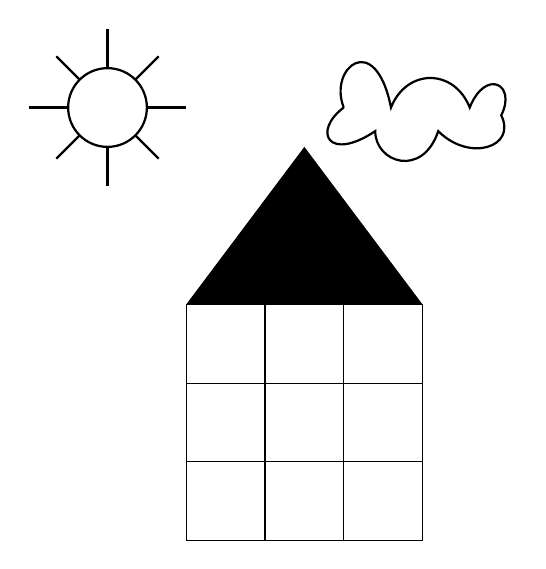
\begin{tikzpicture}
            % Das Dach des Hauses
            \fill[black] (0,0) -- (1.5,2) -- (3,0) -- cycle;

            % Das Raster unter dem Dach (Haus)
            \draw (0,0) rectangle (3,-3);
            \foreach \x in {1,2} {
                    \draw (\x,0) -- (\x,-3); % Vertikale Linien
                    \draw (0,-\x) -- (3,-\x); % Horizontale Linien
                }

            % Sonne
            \draw[thick] (-1,2.5) circle (0.5); % Gesicht
            \draw[thick] (-1,3) -- (-1,3.5); % Strahlen oben
            \draw[thick] (-1.5,2.5) -- (-2,2.5); % Strahlen links
            \draw[thick] (-0.5,2.5) -- (0,2.5); % Strahlen rechts
            \draw[thick] (-1,2) -- (-1,1.5); % Strahlen unten
            \draw[thick] (-1.35,2.85) -- (-1.65,3.15); % Schräge Strahlen
            \draw[thick] (-0.65,2.85) -- (-0.35,3.15);
            \draw[thick] (-1.35,2.15) -- (-1.65,1.85);
            \draw[thick] (-0.65,2.15) -- (-0.35,1.85);
            %\draw[thick] (-1.2,2.7) arc[start angle=180,end angle=359,radius=0.2]; % Lächeln

            % Wolke
            \draw[thick] (2,2.5) .. controls (1.8,3) and (2.4,3.5) .. (2.6,2.5)
            .. controls (2.8,3) and (3.4,3) .. (3.6,2.5)
            .. controls (3.8,3) and (4.2,2.8) .. (4,2.4)
            .. controls (4.2,2) and (3.6,1.8) .. (3.2,2.2)
            .. controls (3,1.6) and (2.4,1.8) .. (2.4,2.2)
            .. controls (1.8,1.8) and (1.6,2.2) .. (2,2.5);

        \end{tikzpicture}
    \end{center}

    \vspace{7cm}


\end{bsp}
\clearpage

\begin{ueb}
    {Vermischte Aufgaben}{}
    \begin{enumerate}

        % Kombinatorik
        \item Wie viele Möglichkeiten gibt es, 3 Eintrittskarten fürs Theater an 5 Personen zu verschenken, wenn\dots
              \begin{enumerate}
                  \item Jede Person höchstens eine Karte erhalten kann und die Sitzplätze nummeriert sind?
                  \item Jede Person auch mehrere Karten erhalten kann und die Sitzplätze nummeriert sind?
                  \item Jede Person höchstens eine Karte erhalten kann und die Sitzplätze nicht nummeriert sind?
                  \item Jede Person auch mehrere Karten erhalten kann und die Sitzplätze nicht nummeriert sind?
              \end{enumerate}

        \item Der firmeneigene Parkplatz hat für 15 Autos Platz. Auf wie viel Arten können die Plätze besetzt werden, wenn 12 Kunden ihre Autos parkieren wollen?

        \item Wie viele verschiedene Flaggen mit drei Längsstreifen (rot, blau oder weiss) gibt es, falls jeder Streifen eine andere Farbe haben soll?


        \item Aus 12 Italienern, 13 Österreichern, 7 Franzosen und 5 Schweizern wird ein Siebnerkomitee ausgewählt. Wie viele Möglichkeiten hat man dabei, wenn in dem Komitee 2 Italiener, 2 Österreicher, 2 Franzosen und 1 Schweizer sein sollen?

        \item Neun Blumenstöcke sollen in eine Reihe gestellt werden. Es handelt sich um 4 gelbe, 3 rote und 2 weisse Blumenstöcke. Auf wie viele Arten kann ich die Stöcke anordnen?

        \item
              \begin{enumerate}
                  \item Auf wie viele Arten kann man 5 rote Gummibärchen auf 8 Kinder verteilen, wenn kein Kind mehrere als einen Bär erhalten soll?
                  \item Auf wie viele Arten kann man 8 rote Gummibärchen auf 5 Kinder verteilen, wenn jedes Kind mindestens einen Bär erhalten soll?
              \end{enumerate}


        \item Auf wie viele Arten kann man 8 Türme auf ein Schachbrett stellen, die sich gegenseitig nicht schlagen?
              \begin{center}
                  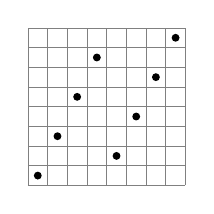
\begin{tikzpicture}[scale=0.25]
                      \draw[step=1cm,gray,very thin] (0,0) grid (8,8);
                      \foreach \x/\y in {0/0, 1/2, 2/4, 3/6, 4/1, 5/3, 6/5, 7/7} {
                              \fill (\x+0.5,\y+0.5) circle (0.2);
                          }
                  \end{tikzpicture}
              \end{center}


        \item Sechs verschieden gefärbte Kugeln sollen in 10 durchnummerierte Kästchen gelegt werden, wobei in einem Kästchen höchstens eine Kugel liegen darf. Wie viele Arten, die Kugeln unterzubringen, gibt es?


        \item
              Wie viele verschiedene, achtstellige Zahlenreihen können aus den Ziffern 3, 3, 4, 4, 4, 5, 5 und 7 gebildet werden?



        \item In einem Lokal sind noch 5 Stühle frei. Auf wie viele Arten können diese genutzt werden, wenn 3 (5, 8) Gäste gleichzeitig ankommen und wenn interessiert, wer auf welchem Stuhl sitzt?




              % Wahrscheinlichkeiten (und Kombinatorik )
        \item Sechzehn Pferde nahmen an einem Rennen teil. Alice gibt eine Dreierwette (= Voraussage der ersten drei Plätze in der richtigen Reihenfolge) zufällig ab. Wie gross ist die Wahrscheinlichkeit, dass sie gewinnt?

        \item Fünf Briefe werden zufällig in fünf adressierte Couverts gesteckt. Wie gross ist die Wahrscheinlichkeit, dass sich mindestens vier Briefe im richtigen Couvert befinden?





        \item Auf wie viele Arten kann man 5 Frauen und 5 Männer in eine Reihe stellen, falls \dots
              \begin{enumerate}
                  \item \dots die Reihenfolge egal ist,
                  \item \dots nie 2 Frauen oder 2 Männer nebeneinander stehen,
                  \item \dots alle Frauen nebeneinander stehen?
                  \item Die Position in der Reihe wird zufällig vergeben. Mit welcher Wahrscheinlichkeit stehen Alice und Bob nebeneinander?
              \end{enumerate}

        \item Für die Verbindung mit dem Beamer wählt das Gerät zufällig vier Ziffern, die der Benutzer eingeben muss. Wie gross ist die Wahrscheinlichkeit, dass mindestens zwei der Ziffern gleich sind.

        \item Auf Beginn des Schuljahres kehren zwölf Jugendliche aus dem Austausch zurück und müssen auf die bereits bestehenden Klassen verteilt werden. Vier der Schüler*innen kommen in die Klasse 3a, drei in Klasse 3b und die restlichen in die Klasse 3c. Unter den zwölf Rückkehrer*innen sind auch Alice und Bob.
              Wie gross ist die Wahrscheinlichkeit, dass sie in die gleiche Klasse kommen, wenn die Zuteilung zufällig erfolgt?

        \item Alice wirft achtmal eine Münze und notiert das Ergebnis. Sie schreibt K für einen Kopfwurf und Z für einen Zahlwurf. KZZZKZKK wäre zum Beispiel ein Ergebnis.

              Mit welcher Wahrscheinlichkeit treten gleich viele Kopf- wie Zahlwürfe auf?

        \item Mit welcher Wahrscheinlichkeit %erhält man beim Yahtzee in einem Wurf eine grosse Strasse, das heisst 
              bei einem Wurf mit fünf Würfeln fünf aufeinanderfolgende Zahlen?

        \item Beim Sporttoto sind jeweils 13 Spielausgänge vorauszusagen. Ein einzelnes Spiel kann die Ausgänge 1, 2 oder x haben. Bob füllt den Totoschein zufällig aus. Mit welcher Wahrscheinlichkeit wird er bis auf zwei Spiele alles richtig vorhersagen (sog. 'Elfer')? Wie gross ist die Wahrscheinlichkeit für einen 'Zehner'?

    \end{enumerate}
\end{ueb}

\clearpage

\emph{Lösungen}
\begin{enumerate}
    \item
          \begin{enumerate}
              \item 60
              \item 125
              \item 10
              \item 35
          \end{enumerate}

    \item \(2.18 \cdot 10^{11}\)
    \item 6
    \item 540540
    \item 1260
    \item  \begin{enumerate}
              \item 56
              \item 35
          \end{enumerate}
    \item 40320
    \item 151200
    \item 1680
    \item 60; 120; 6720
    \item \(\frac{1}{3360}\)
    \item \(\frac{1}{120}\)

    \item \begin{enumerate}
              \item 3628800
              \item 28800
              \item 86400
              \item \(\frac{725760}{3628800}=20\% \)
          \end{enumerate}
    \item \(P(\text{mindestens zwei gleiche Ziffern}) = 1 - P(\text{alles unterschiedliche Ziffern}) = 1- \frac{5040}{10000} =0.496 \)
    \item \(\frac{2520 + 1260 + 4200}{27720} = \frac{7980}{27720} \approx 28.78 \% \)
    \item \(\frac{70}{256} \approx 27.34 \% \)
    \item \(\frac{2\cdot 5!}{7776} \approx 3.08 \% \)
    \item \(P (\text{Elfer})=\frac{\binom{13}{11} \cdot 2^2 }{3^{13}} \approx 0.02 \% ; \quad
          P(\text{Zehner})= \frac{\binom{13}{10} \cdot 2^3 }{3^{13}} \approx 0.14 \% \)
\end{enumerate}









\clearpage



\begin{ueb}
    {Der sichere Gewinn?}{}
    Kann man unter Umständen beim Zahlenlotto mit Sicherheit gewinnen?

    Beim Schweizer Zahlenlotto muss man 6 verschieden Zahlen zwischen 1 und 42 ankreuzen. Zusätzlich muss pro Tipp eine Glückszahl zwischen 1 und 6 angekreuzt werden. Bei der Ziehung werden die 6 Gewinnzahlen und die Gewinn-Glückszahl ermittelt. Je mehr richtige Zahlen man angekreuzt hat, desto höher fällt der Gewinn aus. Die durchschnittlichen Gewinnsummen sind:

    % \begin{table}[ht]
    \begin{center}


        \begin{tabular}{@{}ll@{}}
            \toprule
            \textbf{Anzahl richtige Zahlen} & \textbf{Gewinnsumme} \\ \midrule
            6 Richtige und Glückszahl       & Jackpot              \\
            6 Richtige                      & 1'000'000.-          \\
            5 Richtige und Glückszahl       & 5'000.-              \\
            5 Richtige                      & 1'000.-              \\
            4 Richtige und Glückszahl       & 150.-                \\
            4 Richtige                      & 75.-                 \\
            3 Richtige und Glückszahl       & 25.-                 \\
            3 Richtige                      & 10.-                 \\ \bottomrule
        \end{tabular}
        % \caption{Gewinnsummen für die verschiedenen Kombinationen richtiger Zahlen}
        %     \label{tab:gewinnsummen}
        % \end{table}

    \end{center}
    Die Höhe des Jackpots hängt davon ab, wie lange er nicht geknackt wurde. Im Dezember 2016 lag der bisher höchste Betrag von 70 Millionen Franken im Jackpot.

    Bob behauptet, dass es sich bei sehr hohen Jackpots lohnt, alle möglichen Tipps auszufüllen. Wir wollen nachrechnen, ob er recht hat, und wie gross der Jackpot sein müsste:

    \begin{enumerate}
        \item Ein Tipp kostet 2.50. Wie viel würde es kosten, alle möglichen Tipps abzugeben?

        \item Angenommen, man hat alle Tipps abgegeben.
              \begin{enumerate}
                  \item Wie viele ``6er mit Glückszahl'' sind dabei?
                  \item Wie viele ``6er ohne Glückszahl'' sind dabei?
                  \item Berechnen Sie die Anzahl ``5er mit Glückszahl'' (Also solche Tipps mit 5 richtigen und einer falschen Zahl mit richtiger Glückszahl).
                  \item Bestimmen Sie auch, wie viele andere Gewinne (5er ohne Glückszahl bis 3er) dabei sind.
              \end{enumerate}

        \item Wie gross müsste der Jackpot sein, damit es sich lohnt, alles auszufüllen?

        \item Geben Sie mögliche Gründe an, wieso es sich auch in diesem Fall nicht lohnen würde, alle Tipps abzugeben.
    \end{enumerate}
\end{ueb}

\clearpage

\begin{ueb}
    {Roberto geht zur Arbeit\dots}{}
    \begin{center}
        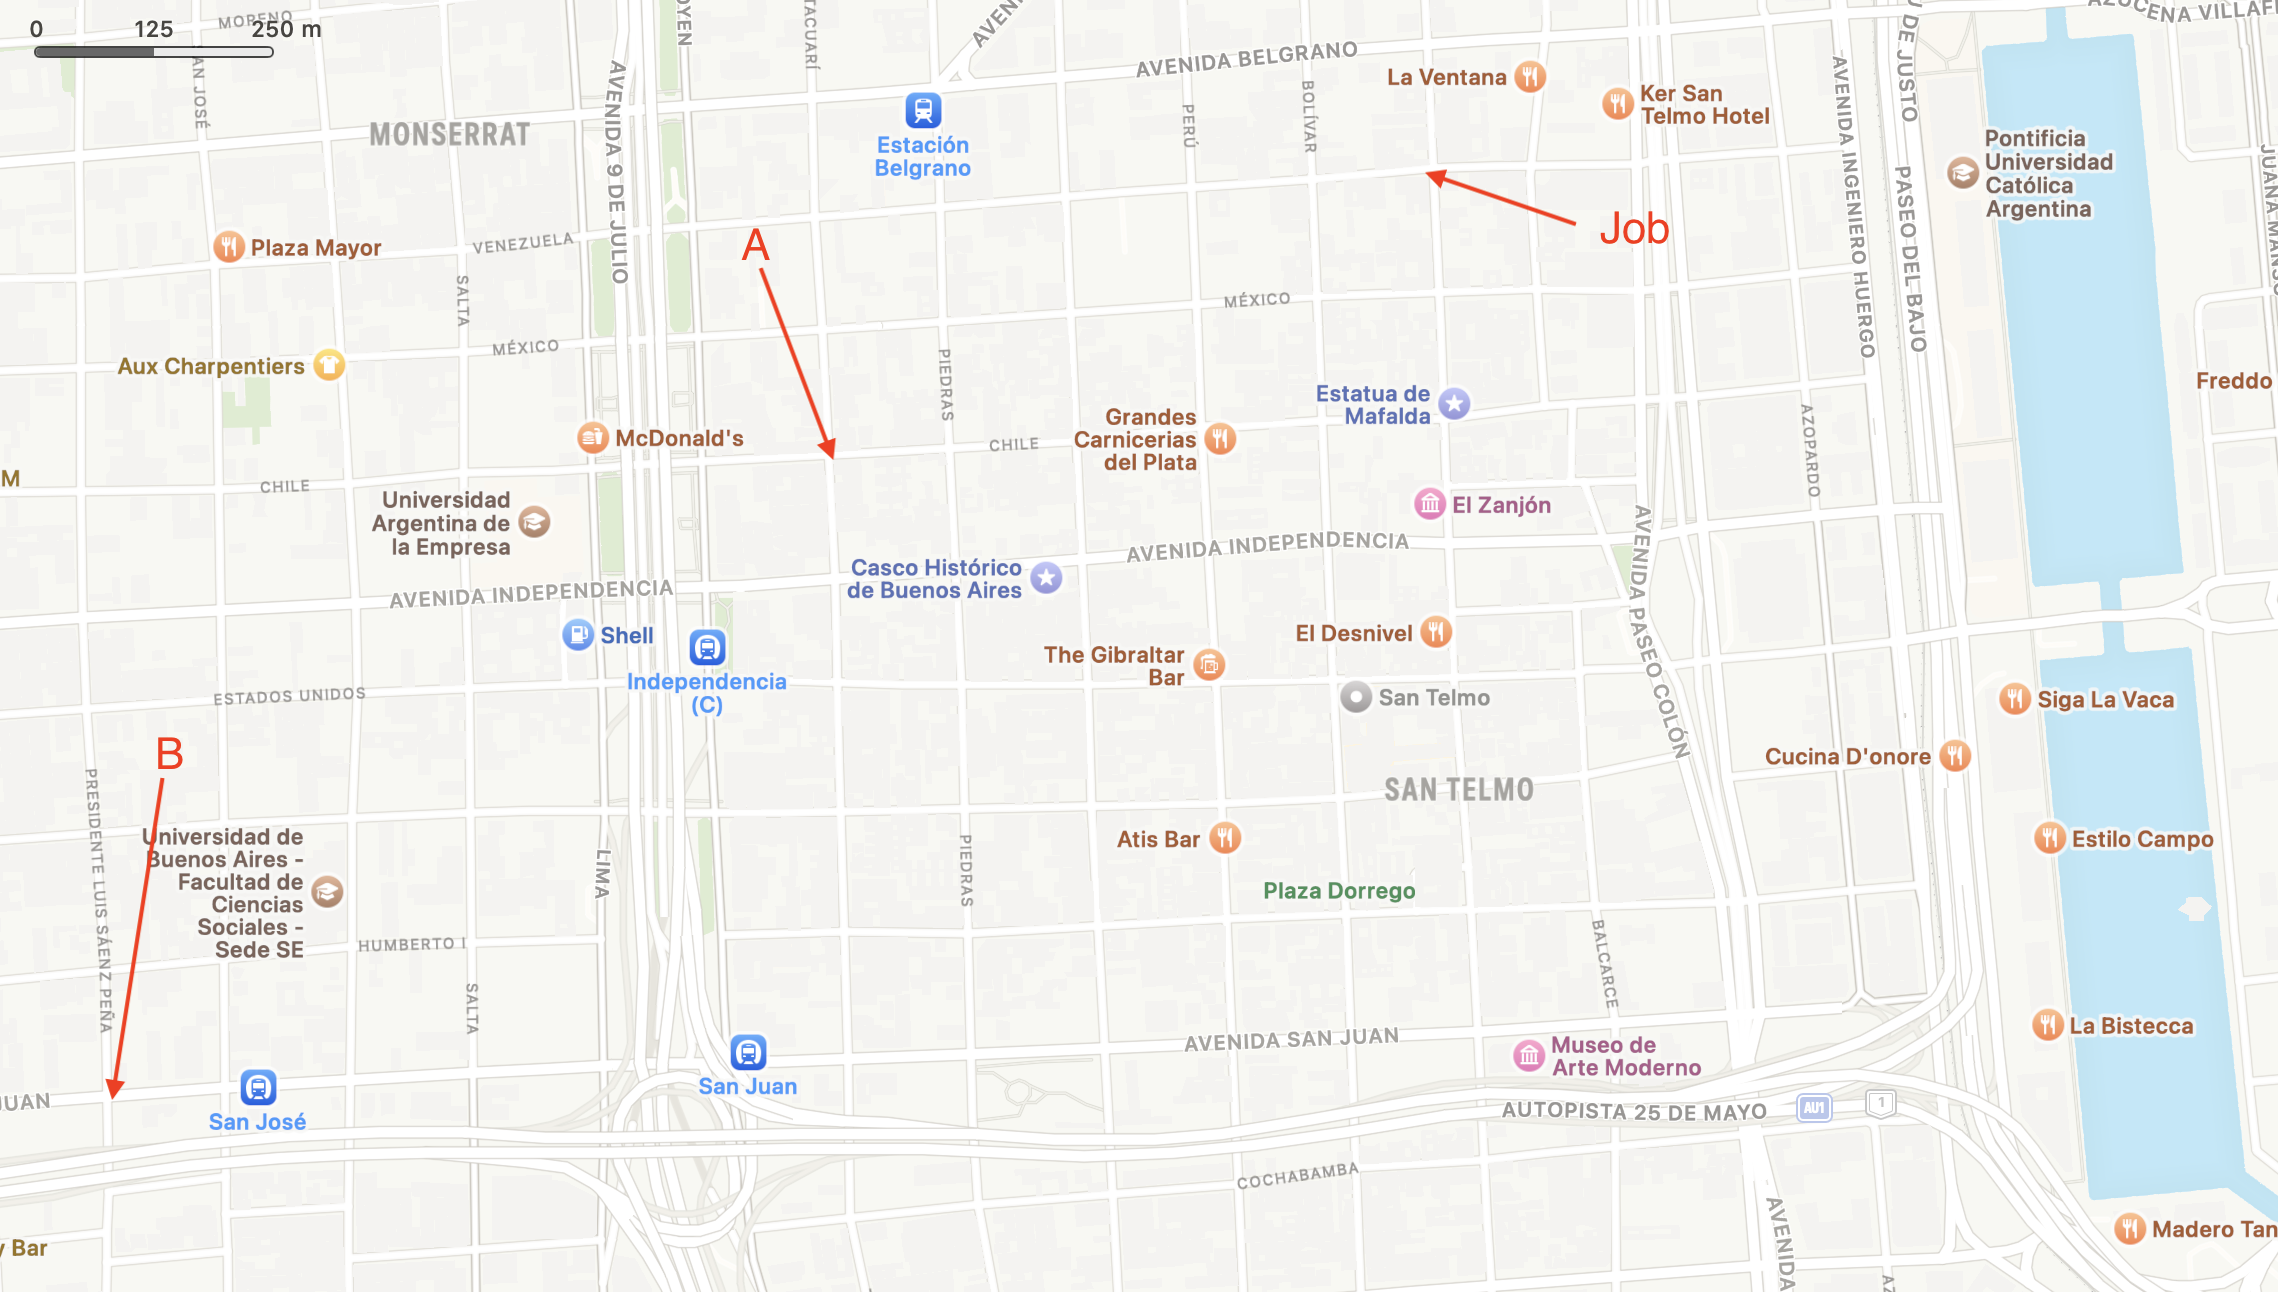
\includegraphics[width = \textwidth]{media/BuenosAires.png}
    \end{center}
    Die Abbildung oben zeigt einen Ausschnitt aus der Strassenkarte von Buenos Aires.

    Roberto (genannt Bob) arbeitet an 250 Tage pro Jahr. Jeden Tag wählt er einen neuen Arbeitsweg von seinem Wohnort (B) zu Arbeitsort (Job), macht dabei aber keine Umwege und bewegt sich nur entlang der Hauptstrassen (ganz kleine Wege auf der Karte nicht beachten).

    \begin{enumerate}
        \item Wie viele Jahre dauert es, bis er alle möglichen Wege abgelaufen ist?

              Achtung: Die Avenida 9 de Julio lässt sich an einer Stelle nicht queren! Taktik: Berechnen Sie die Anzahl Wege, wenn die Querung auch an dieser Stelle möglich wäre. Ziehen Sie dann alle Wege ab, welche über die nicht vorhandene Querung verlaufen.

              %(Kontrolle: Es sind 27204 Wege --> 108.8 Jahre )

        \item Bonus: Wie viele Jahre dauert es, wenn er nur Wege wählt, die an Alicias (A) Haus vorbeiführen?

    \end{enumerate}

\end{ueb}










\clearpage
\subsection{Der binomische Lehrsatz}
Seit der ersten Klasse wissen wir: Will man den Term \((a+b)^4\) ausmultiplizieren, kann man auf das pascalsche Dreieck zurückgreifen:

\[
    \begin{array}{ccccccccc}
          &   &   &   & 1 &   &   &   &   \\
          &   &   & 1 &   & 1 &   &   &   \\
          &   & 1 &   & 2 &   & 1 &   &   \\
          & 1 &   & 3 &   & 3 &   & 1 &   \\
        1 &   & 4 &   & 6 &   & 4 &   & 1
    \end{array}
\]

Die Zahlen in der letzten Zeile entsprechen den Koeffizienten der Monome in \((a+b)^4\). Das heisst:
\[
    (a+b)^4 = 1 \cdot a^4 + 4 \cdot a^3 b + 6 \cdot a^2 b^2 + 4 \cdot ab^3 + 1 \cdot b^4
\]

In diesem Abschnitt werden wir folgende Fragen rund um das pascalsche Dreieck beantworten:
\begin{itemize}
    \item Gibt es einen bequemeren Weg, wie man den Koeffizienten von z.\,B. \(a^7 b^5\) im Term \((a+b)^{12}\) berechnen kann? (Ohne zuerst die 12 Zeilen des Dreiecks auszurechnen)
    \item Wie kann man den Koeffizienten von \(a^5 b^6 c^3\) in \((a+b+c)^{14}\) ohne grossen Aufwand angeben?
    \item Wieso eigentlich liefert das pascalsche Dreieck die richtigen Koeffizienten?
\end{itemize}



\begin{LA}
    {}{}
    Bob berechnet Potenzen von \((a+b)\) rein nach der Regel ``jede mit jede'':


    \[
        (a+b)(a+b) = aa + ab + ba + bb
    \]

    \[
        (a+b)(a+b)(a+b) = aaa + aab + \cdots
    \]

    \begin{enumerate}
        \item Führen Sie die zweite Rechnung nach diesem Prinzip zu Ende.
        \item Berechnen Sie auf diese Art auch \((a+b)(a+b)(a+b)(a+b)\).
        \item Der Koeffizient (= Vorfaktor) von \(a^3 b\) in \((a+b)^4\) ist 4, weil \(aaab + aaba + abaa + baaa = 4a^3 b\) ist. Welches ist der Koeffizient von \(a^2 b^2\)?
        \item Wie lautet der Koeffizient von \(a^7 b^5\) im Term \((a+b)^{12}\)?
    \end{enumerate}

\end{LA}

\clearpage

Aus der Einführungsaufgabe folgt:

\begin{satz}
    {Binomischer Lehrsatz}{binomLehrsatz}
    Für jede natürliche Zahl \(n\) gilt:

    \[
        (a+b)^n = \binom{n}{0} a^0 b^n + \binom{n}{1} a^1 b^{n-1} + \binom{n}{2} a^2 b^{n-2} + \cdots + \binom{n}{n-1} a^{n-1} b + \binom{n}{n} a^n b^0
    \]

    oder mit dem Summenzeichen:

    \[
        (a+b)^n = \sum_{k=0}^n \binom{n}{k} a^k b^{n-k}.
    \]
\end{satz}

\textbf{Bemerkung:} Aus diesem Grund heissen Zahlen der Form \(\binom{n}{k}\) \textit{Binomialkoeffizienten}.


Zum Schluss wollen wir noch erklären, wieso die Methode mit dem pascalschen Dreieck, die wir bisher immer verwendet haben, die richtigen Koeffizienten liefert.

Dazu müssen wir zeigen, dass die Zahlen, die man erhält, wenn man beginnt mit:
\[
    \begin{array}{ccc}
          & 1 &   \\
        1 &   & 1 \\
    \end{array}
\]
und dann weiterfährt, indem man immer die Summe zweier benachbarten Zahlen darunter schreibt

\[
    \begin{array}{ccccccccc}
          &   &   &   & 1 &   &   &   &   \\
          &   &   & 1 &   & 1 &   &   &   \\
          &   & 1 &   & 2 &   & 1 &   &   \\
          & 1 &   & 3 &   & 3 &   & 1 &   \\
        1 &   & 4 &   & 6 &   & 4 &   & 1
    \end{array}
\]

genau den Binomialkoeffizienten

\[
    \begin{array}{ccccccccc}
                     &              &              &              & \binom{0}{0} &              &              &              &              \\
                     &              &              & \binom{1}{0} &              & \binom{1}{1} &              &              &              \\
                     &              & \binom{2}{0} &              & \binom{2}{1} &              & \binom{2}{2} &              &              \\
                     & \binom{3}{0} &              & \binom{3}{1} &              & \binom{3}{2} &              & \binom{3}{3} &              \\
        \binom{4}{0} &              & \binom{4}{1} &              & \binom{4}{2} &              & \binom{4}{3} &              & \binom{4}{4}
    \end{array}
\]
erhält.

Der erste Teil ist schnell gemacht. Tatsächlich sind die obersten drei Zahlen \(\binom{0}{0} = 1\), \(\binom{1}{0} = 1\) und \(\binom{1}{1} = 1\). Das pascalsche Dreieck beginnt also richtigerweise mit:

\[
    \begin{array}{ccc}
          & 1 &   \\
        1 &   & 1 \\
    \end{array}
\]

Das mit der Summe ist etwas anspruchsvoller. Wir müssen zeigen, dass die Summe zweier benachbarten Zahlen im Dreieck mit den Binomialkoeffizienten die darunterliegende Zahl ergibt.

So muss beispielsweise
\[
    \binom{5}{2} + \binom{5}{3} = \binom{6}{3}
\]
gelten.

Allgemein müssen wir zeigen, dass
\[
    \binom{n}{k-1} + \binom{n}{k} = \binom{n+1}{k}.
\]

Im Folgenden wird diese Formel auf zwei verschiedene Arten begründet.

\begin{enumerate}
    \item \textbf{Der intuitive Weg:}

          Ein Lehrer und eine Klasse mit 23 Schüler*innen möchten Fussball spielen.
          \begin{enumerate}
              \item Auf wie viele Arten können sie ein Team mit 11 Spieler*innen bilden, wenn der Lehrer mitspielen darf?
              \item Auf wie viele Arten können sie ein Team mit 11 Spieler*innen bilden, wenn der Lehrer mitspielen \textbf{muss}?
              \item Auf wie viele Arten können sie ein Team mit 11 Spieler*innen bilden, wenn der Lehrer \textbf{nicht} mitspielen darf? Lösen Sie die Aufgabe, ohne das Resultat aus b) zu verwenden!
              \item Berechnen Sie nochmals die Möglichkeiten von Aufgabe a), indem Sie die Resultate von b) und c) verwenden. Was für eine Formel ergibt sich?
              \item Wie lautet die Formel, wenn die Klasse aus \(n\) SchülerInnen besteht und das Team aus \(k\) Spieler*innen bestehen soll?
          \end{enumerate}
    \item \textbf{(Challenge) Der algebraische Weg:}

          Schreiben Sie die Formel
          \[
              \binom{n}{k-1} + \binom{n}{k} = \binom{n+1}{k}
          \]
          nochmals auf, indem Sie die Binomialkoeffizienten als Quotienten von Fakultätszahlen schreiben, also
          \[
              \binom{n}{k} = \frac{n!}{k! \cdot (n-k)!}.
          \]

          Beweisen Sie durch geschicktes Umformen, dass die Formel stimmt.

\end{enumerate}





\clearpage
\begin{ueb}
    {}{}
    \begin{enumerate}
        \item Bestimmen Sie den Koeffizienten von \(a^3b^9\) in \((a+b)^{12}\).
        \item Bestimmen Sie den Koeffizienten von \(a^k b^{k-1}\) in \((a-b)^{15}\)
        \item Bestimmen Sie den Koeffizienten von \(a^{14} b^{k}\) in \((a^2+b)^{10}\)
        \item Erklären Sie, wieso der Koeffizient von \(a^5 b^6 c^3\) in \((a+b+c)^{14}\) genau 168'168 ist.
        \item Beweisen Sie, dass \(\binom{n}{0} + \binom{n}{1} + \binom{n}{2} + \cdots + \binom{n}{n} = 2^n\) ist.
    \end{enumerate}

\end{ueb}

\clearpage
\emph{Lösungen}
\begin{enumerate}
    \item 220
    \item \(-6435\)
    \item 120
    \item \(\binom{14}{5}\cdot \binom{9}{6} = 168168\)
    \item Setze \(a=1\) und \(b=1\) in den binomischen Lehrsatz ein\dots
\end{enumerate}







